\documentclass[a4paper,italian,12pt]{book}
\usepackage[utf8]{inputenc}
\usepackage[italian]{babel}
\usepackage[T1]{fontenc}
\usepackage [a4paper,left=2.5cm,bottom=3cm,right=2.5cm,top=3cm]{geometry}
\usepackage{graphicx} % the demo option is just for the example
\usepackage{amssymb}
\usepackage{titling}
%\usepackage{fontspec}

\pretitle{%
  \begin{center}
  \LARGE
  
\includegraphics[scale=0.2]{Figure/logo.jpg}\\[\bigskipamount]
}
\posttitle{\end{center}}
\title{MANUALE GESTIONE PROTOCOLLO}
\author{Raucci Antonio}
\date{ver. 1.2}

\begin {document} 
\maketitle
\tableofcontents

\newpage 
\null\vspace{\stretch{1}}
\begin{flushright}
\textit{Al Direttore dei Servizi Generali ed Amministrativi \\ Alessandrini Savina}
\end{flushright}
\vspace{\stretch{2}}\null

\chapter{Istruzioni Operative}
\section{Gestione Protocollo}
Operazione giornaliera:
%\begin{enumerate}
Controllo posta elettronica da Miur.it \\
\\
\textit{Accesso $\to$ webmail@istruzione.it} \\
\\
Con credenziali: \\
\\
Username RMIS112007 \\
Password xxxxx \\

Si verifichi che l'utilizzo della mailbox sia al di sotto del $50\%$. Nel caso la percentuale fosse più alta, si proceda alla cancellazione delle e-mail a partire da quelle più vecchie.

Si fa presente che le e-mail vengono duplicate da segreteria digitale ma è sconsigliata la cancellazione dalla casella Miur fino a quando non verranno lavorate su segreteria digitale.

E' stato verificato che le e-mail miur-segreteria digitale non vengono sincronizzate immediatamente ma a volte anche dopo varie ore. Pertanto, si consiglia di rivedere sempre se le e-mail precedenti sono state lavorate.
%\end{enumerate}

\section{Segreteria Digitale}
\textit{Specifiche:} 

alla data attuale si ha spazio illimitato per segreteria digitale e 5 gb dedicati per la posta elettronica (sincronizzazione caselle email peo o pec in segreteria digitale).

Una volta che i documenti vengono acquisiti, le e-mail potranno essere cancellate.
Bisogna porre particolare attenzione alla percentuale di riempimento di questo spazio che non dovrà raggiungere il $100\%$ altrimenti non si potranno ricevere ulteriori email.
\\
\\
\section{Lettura Mail}
Per leggere le e-mail è necessario sincronizzarle tramite il comando: \\ricevi posta
\begin{figure}[ht]
\centering

\includegraphics[scale=1]{Figure/ric_posta.jpg} 
%\caption{\label{fig:record-ssl} Processo di elaborazione di un record SSL (overview)}
\end{figure} \\
Poiché nella webmail istruzione le mail in spam non vengono sincronizzate con segreteria digitale, è necessario controllarle manualmente.

\section{Assegnazione Mail}
L'assegnazione può essere effettuata con l'apposito comando: \textit{Assegna} (di seguito illustrato)
\begin{figure}[ht]
\centering
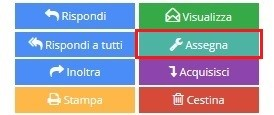
\includegraphics[scale=1]{Figure/ass_mail.jpg} 
%\caption{\label{fig:record-ssl} Processo di elaborazione di un record SSL (overview)}
\end{figure} \\
L'assegnazione di una e-mail può essere effettuata ad un singolo dipendente oppure ad un gruppo di utenti (Es. ad un ufficio: Didattica, Personale, Amministrazione ecc. ecc.).

Le e-mail più importanti verranno prima protocollate e poi assegnate ma fino a che il destinatario (o l'ufficio destinatario) non acquisisce il messaggio, non è possibile effettuare la cancellazione della mail. Non è necessario porre attenzione a questa operazione poiché il simbolo rosso \textit{Cestina} diventerà di un colore più chiaro e non sarà possibile eseguire la cancellazione.

\section{Acquisizione/Protocollo Mail}
Tramite il comando \textit{Acquisisci}
\begin{figure}[ht]
\centering
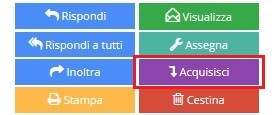
\includegraphics[scale=1]{Figure/prot_mail.jpg} 
%\caption{\label{fig:record-ssl} Processo di elaborazione di un record SSL (overview)}
\end{figure} \\
Si acquisisce l'email e si completano i campi obbligatori:
\\
\\
\\
\\
\begin{itemize}
\item[-] \textit{Tipo documento da caricare:} si specifica a quale area fa riferimento il documento che stiamo acquisendo.
\begin{figure}[ht]
\centering
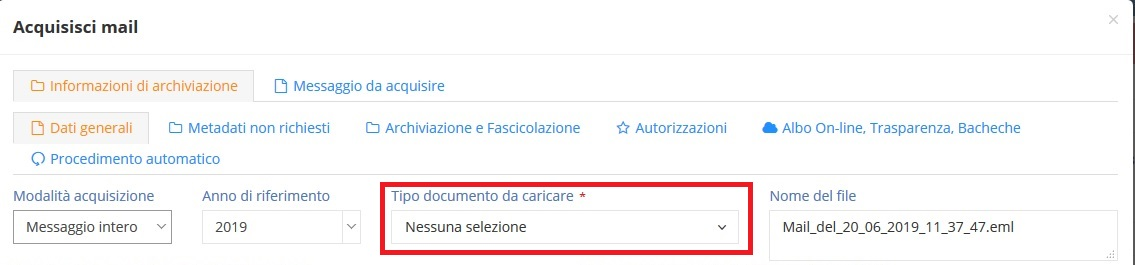
\includegraphics[scale=0.5]{Figure/tipo_doc.jpg} 
%\caption{\label{fig:record-ssl} Processo di elaborazione di un record SSL (overview)}
\end{figure}
\item[-] \textit{Archiviazione e Fascicolazione:} specifica dove verrà archiviato il file effettivamente. Questo dato è variabile: si può riferire sia ad un alunno specifico, scegliendone il nominativo, sia ad una classe intera, scegliendo la classe. Ovviamente possono essere diverse anche le aree scegliendo fascicoli di docenti, personale ata; proprio come avveniva col cartaceo quando si archiviava il foglio nel fascicolo di un dipendente/alunno o all'interno di un faldone generico.
\begin{figure}[ht]
\centering

\includegraphics[scale=0.5]{Figure/arch_fasc_ev.jpg} 
%\caption{\label{fig:record-ssl} Processo di elaborazione di un record SSL (overview)}
\end{figure}
\item[-] \textit{Modalità acquisizione:} indica se deve essere acquisita (o protocollata) tutta l'email (.elm) oppure uno o più allegati, se presenti. Nel caso si voglia protocollare, questo parametro effettua una gestione diversa scegliendo messaggio intero,
\begin{figure}[ht]
\centering
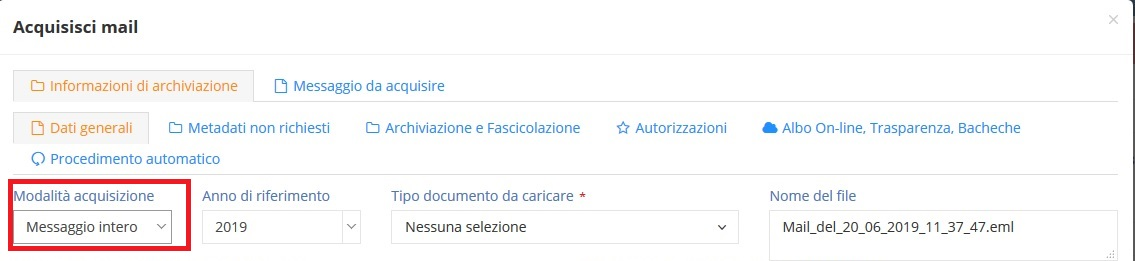
\includegraphics[scale=0.5]{Figure/mod_acquis.jpg} 
%\caption{\label{fig:record-ssl} Processo di elaborazione di un record SSL (overview)}
\end{figure}\\ 
protocolla la mail esterna (.elm) che può contenere uno o più allegati, viceversa, selezionando scelta allegati, verranno protocollati uno o più allegati presenti nella mail.
\begin{figure}[ht]
\centering
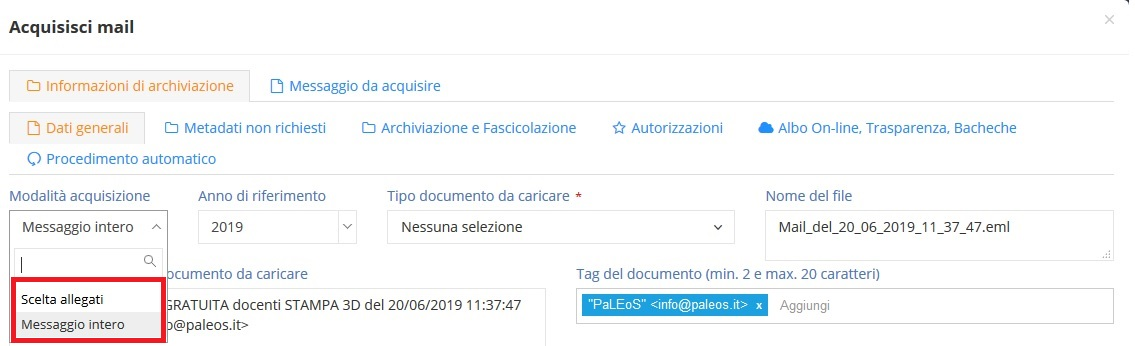
\includegraphics[scale=0.5]{Figure/mod_scelt_all.jpg} 
%\caption{\label{fig:record-ssl} Processo di elaborazione di un record SSL (overview)}
\end{figure} 
\end{itemize} 
\newpage
A questo punto si sceglierà se protocollare il documento oppure acquisirlo senza protocollarlo.

Per acquisire senza protocollare alla voce: \textit{da protocollare} si seleziona \textit{no} e l'operazione è conclusa scegliendo il comando \textit{acquisisci mail}.
\begin{figure}[ht]
\centering
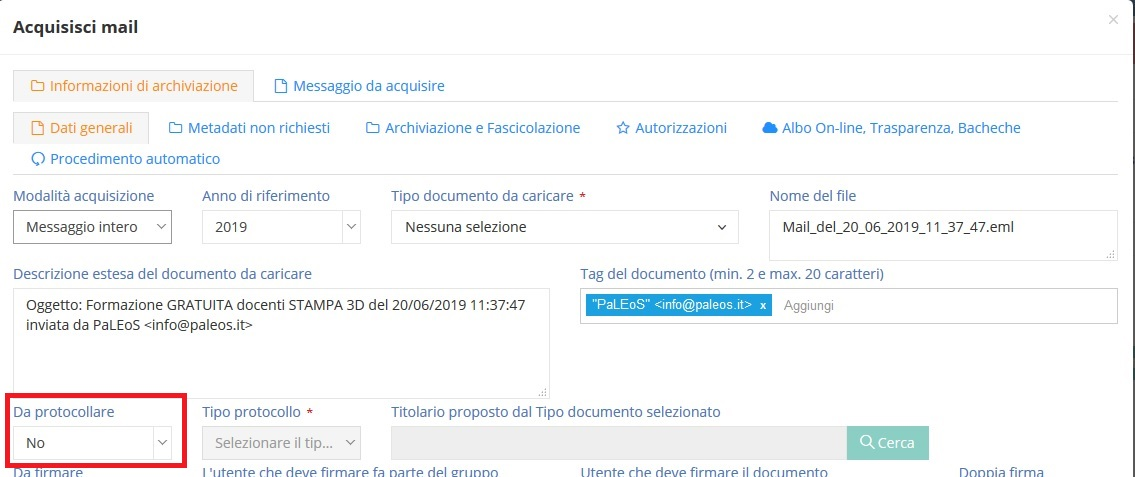
\includegraphics[scale=0.5]{Figure/da_protocollare.jpg} 
%\caption{\label{fig:record-ssl} Processo di elaborazione di un record SSL (overview)}
\end{figure}\\

Nel caso in cui il documento sia da protocollare, si sceglierà la voce \textit{si} oppure \textit{immediato}.
La differenza è che \textit{immediato} farà scegliere il titolario e verrà assegnato il numero di protocollo al termine dell'acquisizione mail mentre scegliendo \textit{si} le scelte verranno rimandate.

Nella fase di acquisizione mail è possibile far firmare il documento dal DS o dal DSGA (tramite la voce da firmare: \textit{si entrambi}) oppure da entrambi scegliendo la voce doppia firma: \textit{SI}.
\begin{figure}[ht]
\centering
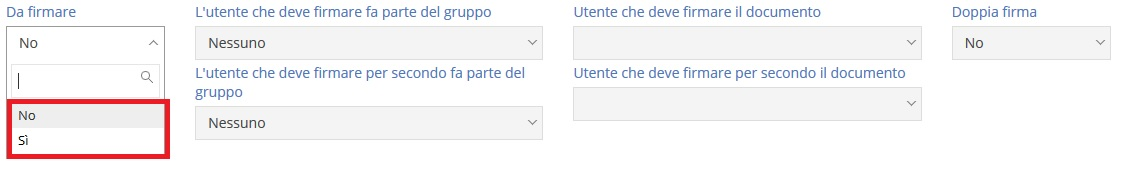
\includegraphics[scale=0.5]{Figure/da_firmare.jpg} 
%\caption{\label{fig:record-ssl} Processo di elaborazione di un record SSL (overview)}
\end{figure} \\

Infine il documento verrà acquisito (e protocollato, se richiesto) tramite il pulsante \textit{acquisisci mail}.

Una volta che la lista email verrà aggiornata, la mail potrà essere assegnata ad un altro dipendente o ufficio.

Poiché lo scopo di utilizzare una segreteria digitale è di evitare che i dipendenti stampino i documenti, il preposto al protocollo NON STAMPERA' i documenti ma li smisterà agli uffici o ai dipendenti destinatari.

Lo stesso iter verrà svolto controllando anche la posta certificata scegliendo in \textit{segreteria digitale $\to$ posta elettronica $\to$ casella mail da gestire $\to$ ricevi posta}.

Anche in questo caso sarà necessario collegarsi alla web mail miur per controllare che la capienza non superi il $50\%$ e si controllano le eventuali email in spam.

\newpage
\section{Cancellazione Email}
Per cancellare le e-mail ci posizioniamo all'ultima pagina scegliendo \textit{ultimo}.
\begin{figure}[ht]
\centering
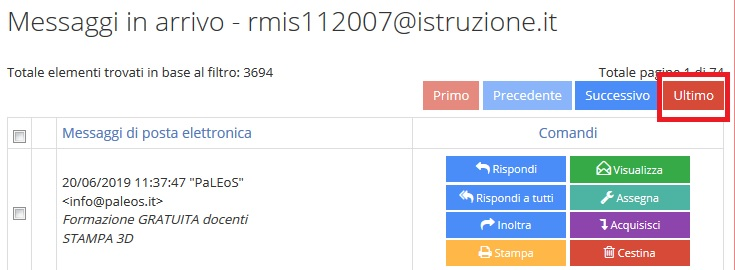
\includegraphics[scale=0.5]{Figure/ultimo.jpg} 
%\caption{\label{fig:record-ssl} Processo di elaborazione di un record SSL (overview)}
\end{figure} \\
Tutte le email acquisite possono essere cancellate poiché sono state già duplicate in segreteria digitale.

Giornalmente potranno essere cancellate anche quelle riguardanti pubblicità informative o comunque che non interessano alla scuola.

\chapter{Conservazione a norma}
La gestione della posta termina inviando in conservazione il file che contiene i protocolli giornalieri al seguente percorso: 

Dalla \textit{Home $\to$ Prow (Protocollo web, icona rossa) }
\begin{figure}[ht]
\centering
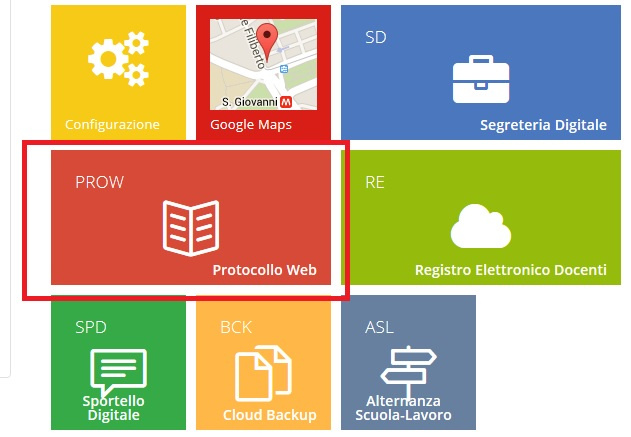
\includegraphics[scale=0.5]{Figure/cons_home.jpg} 
%\caption{\label{fig:record-ssl} Processo di elaborazione di un record SSL (overview)}
\end{figure} \\
\textit{$\to$ Giornaliero}
\begin{figure}[ht]
%\centering
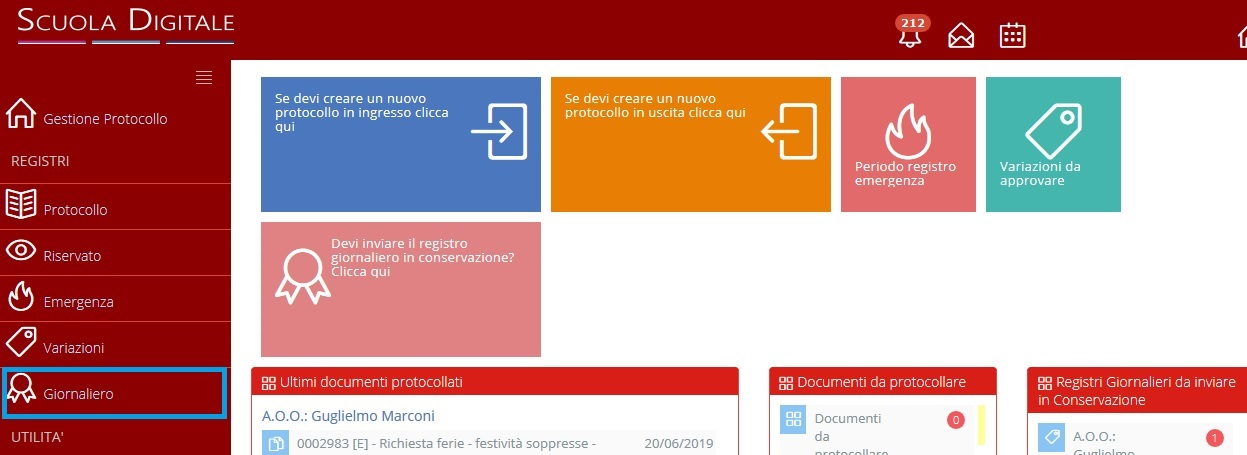
\includegraphics[scale=0.4]{Figure/Giornaliero.jpg} 
%\caption{\label{fig:record-ssl} Processo di elaborazione di un record SSL (overview)}
\end{figure} \\
\\
\\
\\
\\
\\
\\
\textit{$\to$ invio} 
\begin{figure}[ht]
%\centering
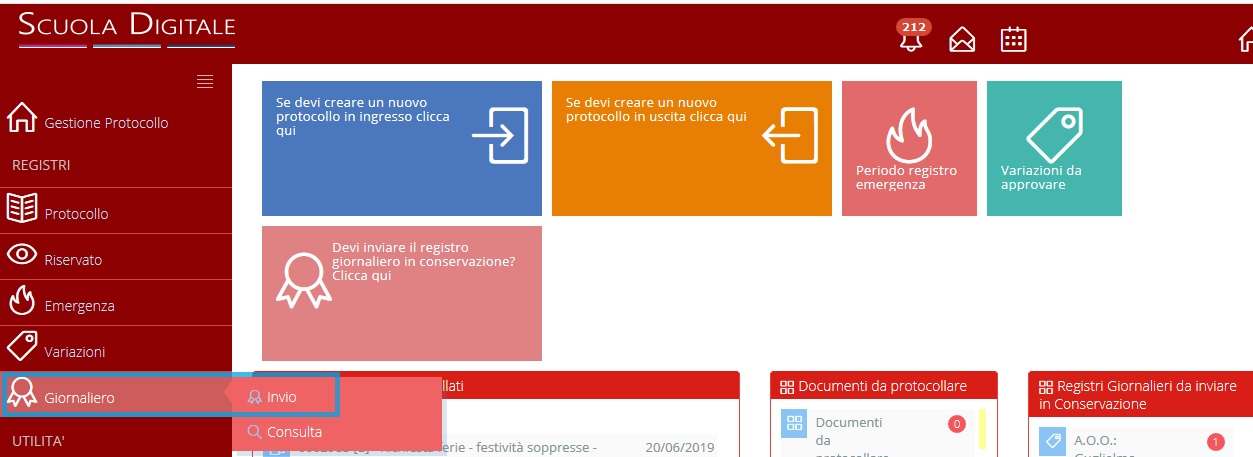
\includegraphics[scale=0.4]{Figure/giorn_invio.jpg} 
%\caption{\label{fig:record-ssl} Processo di elaborazione di un record SSL (overview)}
\end{figure}\\
\textit{$\to$ filtra}\\
\begin{figure}[ht]
\centering
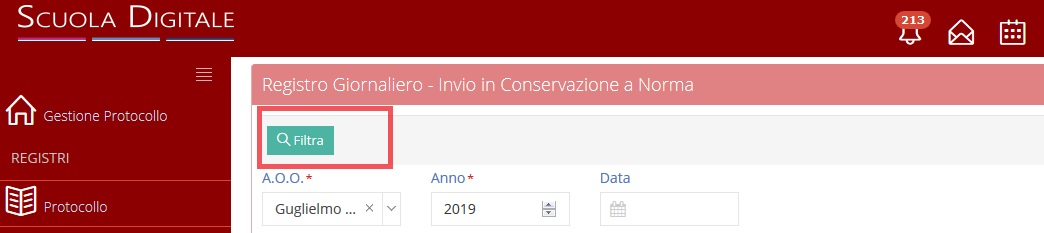
\includegraphics[scale=0.6]{Figure/filtra.jpg} 
%\caption{\label{fig:record-ssl} Processo di elaborazione di un record SSL (overview)}
\end{figure}\\
\textit{ $\to$ invio immediato $\to$ conferma.}
\begin{figure}[ht]
%\centering
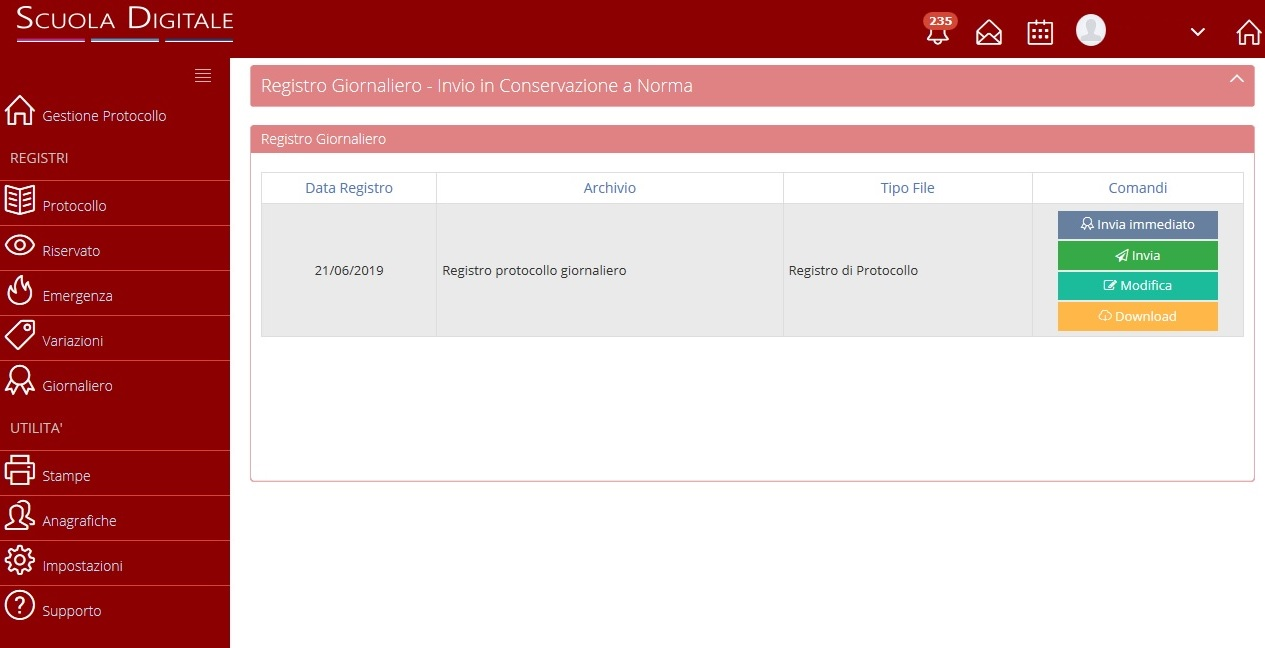
\includegraphics[scale=0.35]{Figure/invio_cons.jpg} 
%\caption{\label{fig:record-ssl} Processo di elaborazione di un record SSL (overview)}
\end{figure} \\
Da giorno successivo è possibile effettuare la convalida del seguente percorso: \\
\textit{SD $\to$ conservazione a norma $\to$ ricerca documenti $\to$ tipo documento: Registro protocollo $\to$ filtra $\to$ Convalida (posto sulla destra)}. Questa operazione può essere svolta anche settimanalmente.
\\
\\
\\
\\
\\
\\
Nel caso in cui l'invio in conservazione fosse stato effettuato verso l'archivio (scelta \textit{invio} e non \textit{invio immediato}), seguire il percorso: \\
\textit{Segreteria digitale $\to$ Conservazione a norma
\begin{figure}[ht]
%\centering
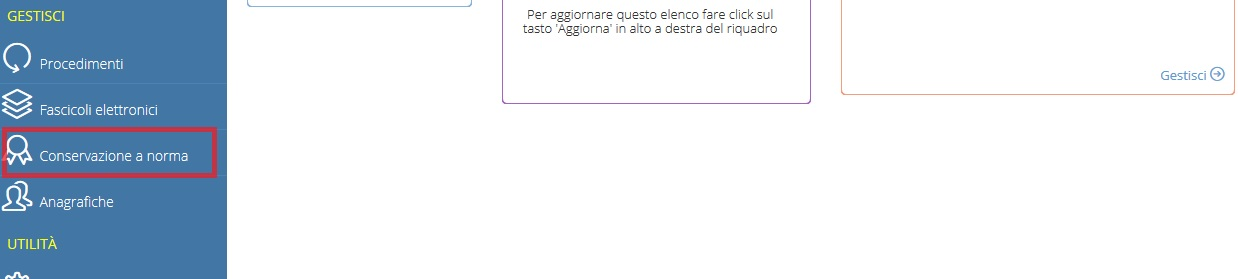
\includegraphics[scale=0.5]{Figure/cons_a_norma.jpg} 
%\caption{\label{fig:record-ssl} Processo di elaborazione di un record SSL (overview)}
\end{figure} \\
$\to$ pacchetto di versamento}
\begin{figure}[ht]
%\centering
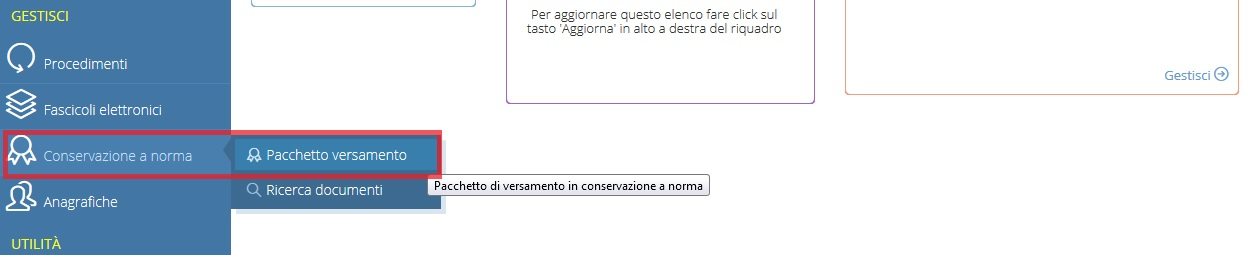
\includegraphics[scale=0.5]{Figure/pacchetto_vers.jpg} 
%\caption{\label{fig:record-ssl} Processo di elaborazione di un record SSL (overview)}
\end{figure}\\ 
\textit{$\to$ tipo documento: registro protocollo} 
\begin{figure}[ht]
%\centering
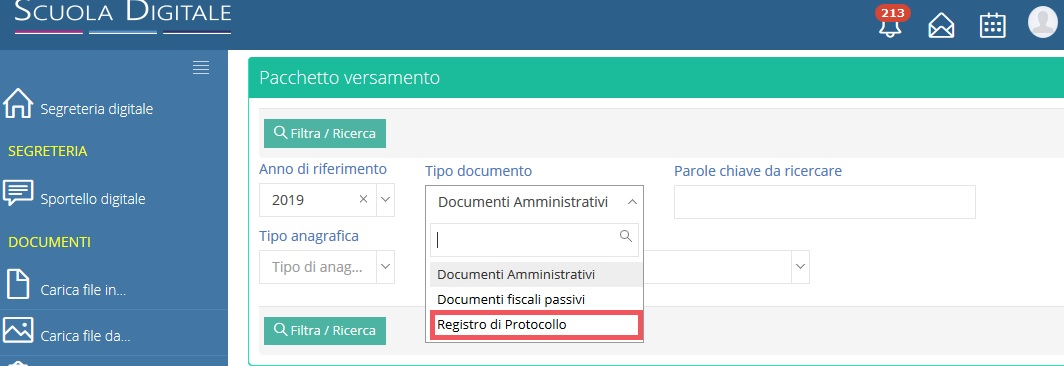
\includegraphics[scale=0.5]{Figure/registro_prot.jpg} 
%\caption{\label{fig:record-ssl} Processo di elaborazione di un record SSL (overview)}
\end{figure}\\
\\
\\
\\
\\
\\
\\
\\
\\
\\
\\
\\
\\
\\
\\
\\
\\
\textit{$\to$ filtra $\to$ selezionare un file per volta}
\begin{figure}[ht]
%\centering
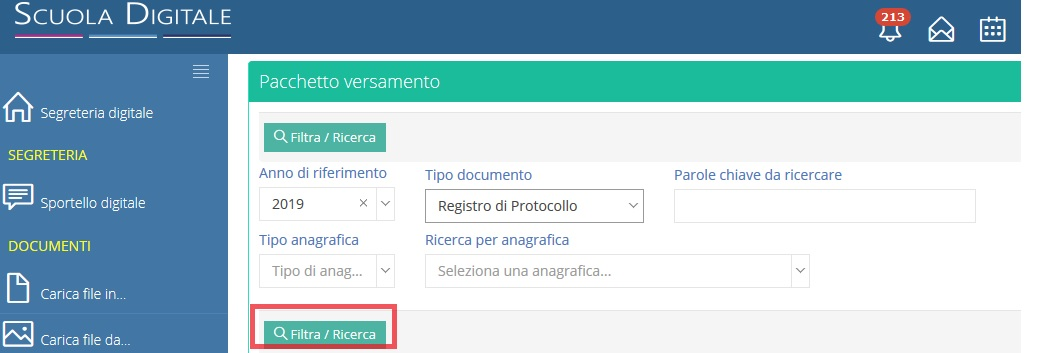
\includegraphics[scale=0.5]{Figure/filtra_pacc_vers.jpg} 
%\caption{\label{fig:record-ssl} Processo di elaborazione di un record SSL (overview)}
\end{figure}\\
\textit{$\to$ invia in conservazione.}
\begin{figure}[ht]
\centering
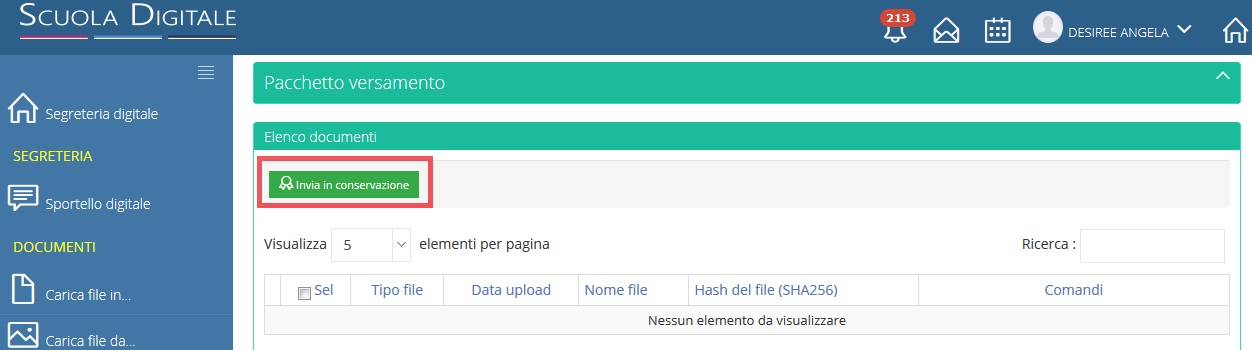
\includegraphics[scale=0.5]{Figure/invia_cons.jpg} 
%\caption{\label{fig:record-ssl} Processo di elaborazione di un record SSL (overview)}
\end{figure}\\

\end {document}
